\chapter{Introduction}
\label{Introduction}
\graphicspath{{Figures/Introduction/}{Figures/Common/}}

%Since their development in 1991, atom interferometers have become competitive in the precision measurement of rotations and gravity gradients with short-term sensitivities of $6 \times 10^{-10} (\text{rad}/\text{s})/\sqrt{\text{Hz}}$ \citep{Gustavson:2000} and $4 \times 10^{-10} (g/\text{m})/\sqrt{\text{Hz}}$ \citep{McGuirk:2002} respectively compared to the world-leading sensitivities of $7\times 10^{-11}(\text{rad}/\text{s})/\sqrt{\text{Hz}}$ \citep{Schreiber:2008} and $10^{-11}(g/\text{m})/\sqrt{\text{Hz}}$ \citep{Moody:1993,Kann:1994}.

Atom interferometry is a young and exciting field.  Since their development in 1991 \citep{Carnal:1991,Keith:1991,Riehle:1991,Kasevich:1991}, atom interferometers have become competitive for the precision measurement of rotations \citep{McGuirk:2002} and gravity gradients \citep{Gustavson:2000}, with sensitivities within about an order magnitude of the best experiments \citep{Schreiber:2008,Moody:1993,Kann:1994}.  For the absolute measurement of the gravitational field strength, atom interferometry is world-leading \citep{Muller:2008}, with sensitivities more than an order of magnitude below that of competing technologies.

In comparison to optical interferometry experiments, which typically use \emph{coherent} optical sources such as (photon) lasers, the above atom interferometry experiments are performed with cold \emph{thermal} atomic sources (the optical equivalent would be black-body radiation).  Coherent sources --- which are characterised by a macroscopic occupation of a single quantum state, and typically have a narrow spectral distribution --- are necessary in optical interferometry experiments in which the interaction time is independent of wavelength, as the measured phase difference depends on the optical frequency and therefore the wavelength.  Sagnac interferometers, gravitational wave sensors, and any interferometer that measures path-length differences are all examples of interferometers that fall into this class.  For atom interferometers however, it is more common that the phase difference for the equivalent experiment (in which the interaction time is also independent of wavelength) will be \emph{independent} of the de Broglie wavelength.  The reason for this difference is due to the different dispersion relations (the expression for energy --- or equivalently, frequency --- as a function of wavenumber) of photons and atoms.  While it is therefore critical that optical interferometers use sources with a narrow range of wavelengths, this is not necessarily the case for atom interferometers.

Coherent atomic sources were developed in 1995 with the achievement of Bose-Einstein Condensation (BEC) in dilute atomic gases \citep{Anderson:1995vn,Bradley:1995ys,Davis:1995}.  Such sources offer several advantages for atom interferometers: a narrower momentum distribution allows better control of systematic uncertainties related to the initial position and velocity; more efficient operation of large-momentum transfer beam splitters, which are highly velocity selective, increasing the interaction time; and quantum degeneracy offers the possibility of increasing sensitivity through the use of squeezed or entangled atomic sources.  Unfortunately, the lower fluxes of currently available coherent atomic sources leads to a higher shot noise, which more than offsets the increases in sensitivity discussed above.  To access these potential advantages of coherent atomic sources, in particular the interesting possibilities involving the use of squeezed and entangled atomic sources (which are interesting in their own right for fundamental tests of quantum mechanics), it will be necessary to produce a truly continuous high-flux source of coherent atoms: the pumped atom laser.  

Pulsed (or quasi-continuous) atom lasers have been produced before.  These are sources of highly degenerate coherent atoms outcoupled from a Bose-Einstein condensate.  These coherent atomic sources are limited by the atom number of the source condensate; once the atoms run out, the atom laser stops.  The condensate must be replenished (or pumped) to produce a truly continuous coherent atomic source.  We focus our attention on this pumping process in this thesis.

% This thesis is primarily motivated at investigating the pumping of an atom laser, but along the way we investigate questions of the beam quality of an atom laser, and interesting effects that occur in outcoupling from a He* condensate.

%10/11 orders of magnitude sensitivity improvement (theoretically).  The same flux cannot be reached.  

%Inertial sensors:  Fundamentally, atoms naturally define an inertial frame.  Falling corner cubes are the most precise for gravimeters.

%Until the development of the `G' ring-laser gyroscope, the atomic Sagnac interferometer \citep{Gustavson:2000} was the most sensitive gyroscope.  The `G' ring-laser gyroscope increased the enclosed area by a factor of 16 over the previously most-sensitive ring-laser gyroscope, C-II.  Larger gyroscopes have run into significant technical problems due to phase noise.

%There are 3 buttons we can push to further the precision of atom interferometers: flux, directionality, and squeezing.  This thesis concentrates on pushing on the `flux' button, which has been shown to be a big win with lasers (and with atom gyroscopes).

%It is hard to underestimate the effect that the laser has had since its invention in 1960 \citep{Maiman:1960}.  Although initially motivated by pure scientific curiosity, its unique properties have given it application in an astonishing array of technologies, in addition to its use as a powerful tool in fundamental research.  

%Laser radiation is distinguished from the light emitted by everyday light sources --- such as light bulbs --- by three main properties, (i) its narrow divergence, (ii) the narrow range of frequencies that are emitted, and (iii) the low intensity noise of the emitted radiation.  Although many applications only make use of the first property, the second property is critical to its use in such applications as laser gyroscopes, gravitational wave detection and fundamental tests of quantum mechanics\footnote{FIXME: Add citations}.  This second property can also be achieved for thermal light through appropriate spectral filtering, however in practice, lasers are a more convenient method for achieving high spectral intensities.  The third property is the true distinguishing property of a laser, however it is only important in specialised applications (e.g.\ gravitational wave detection), in which intensity fluctuations are a significant noise source\footnote{FIXME: In what other circumstances is $g^{(2)}$ important?  It's likely to be important for atom lasers with non-zero interatomic interactions, I suppose.}.

%Quantum mechanics tells us that not only can light behave as a wave, but atoms can too.  This wave nature of atoms is usually indiscernible because the typical wavelength for a thermal atom is many orders of magnitude smaller than the inter-atomic spacing ($\lambda \sim 5 \times\unit[10^{-11}]{m}$ as compared to $d \sim 3 \times\unit[10^{-9}]{m}$).  However, in 1925 Einstein predicted \citep{Einstein:1925} that if a gas of \emph{bosons} (a class of particles which includes many atomic species) was cooled below a critical temperature, a large fraction of the particles would occupy the ground state of the system, forming a coherent wavefunction.  This was achieved in 1995 for dilute atomic gases \citep{Anderson:1995vn,Bradley:1995ys,Davis:1995} with the first production of a Bose-Einstein Condensate (BEC), a macroscopic occupation of atoms in a single spatial mode.  As it is the macroscopic occupation of \emph{photons} in a single spatial mode that gives the optical laser many of its properties, with the achievement of BEC it has become possible to consider the creation of an atomic analogue of the optical laser: the \emph{atom} laser.

%An atom laser, while ideally sharing the above properties of its optical cousin, would behave very differently to an optical laser.  While photons interact strongly with matter, they interact only weakly with themselves or with gravity.  While this makes lasers robust to fluctuations in electromagnetic or gravitational fields, they are therefore less sensitive to these fields in interferometry experiments.  Despite this limitation, optical interferometry has been used in several incredible gravitational experiments, including GRACE, LIGO, and Gravity Probe-A \citep{Vessot:1980}.

%As atoms interact more readily with their environment than photons, atom interferometry has a broad range of applications: to the measurement of electric and magnetic fields in tests of atom and neutron charge neutrality \citep{Arvanitaki:2008}, an application which would be essentially impossible with optical lasers due to the weak photon--photon interaction; to fundamental tests of predictions of General Relativity \citep{Dimopoulos:2007uq}; to the development of gyroscopes \citep{Gustavson:1997}, gradiometers \citep{Snadden:1998,McGuirk:2002} and gravimeters \citep{Peters:2001}, which, while possible using optical lasers, their atomic counterparts are far more compact due to the significantly stronger gravitational interaction.

\section{Photon lasers and Atom lasers}
\label{Introduction:PhotonAndAtomLasers}

The basic features necessary of a continuous atom laser are analogous to the features of a continuous photon laser: a resonator, a lasing mode, an outcoupling process, and a Bose-stimulated pumping mechanism (see \figureref{Introduction:LaserAtomLaserComparison}).  The first three of these features are well understood for an atom laser; experimentally realising the fourth, the pumping mechanism, has presented the greatest challenge.

\begin{figure}
    \centering
    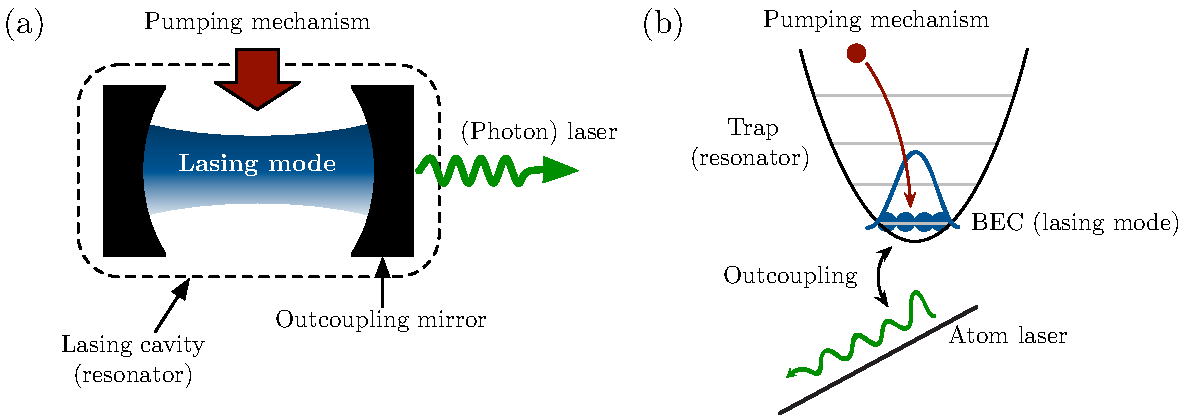
\includegraphics[width=14cm]{LaserAtomLaserComparison}
    \caption{
        \label{Introduction:LaserAtomLaserComparison}
        Schematic diagrams of (a) a photon laser, and (b) an atom laser.
    }
\end{figure}

\subsection{The resonator}

In a photon laser, the resonator is typically a cavity formed between two (or more) mirrors trapping the photons within a region of space.  The optical mode trapped within the resonator is the lasing mode.  For an atom laser, the resonator is an `atom trap', either an optical trap using the ac Stark shift to trap the atoms in a region of high optical intensity, or a magnetic trap using the Zeeman shift to selectively trap certain magnetic hyperfine states near a local minimum of the magnetic field strength.

\subsection{The lasing mode}

\begin{figure}
    \centering
    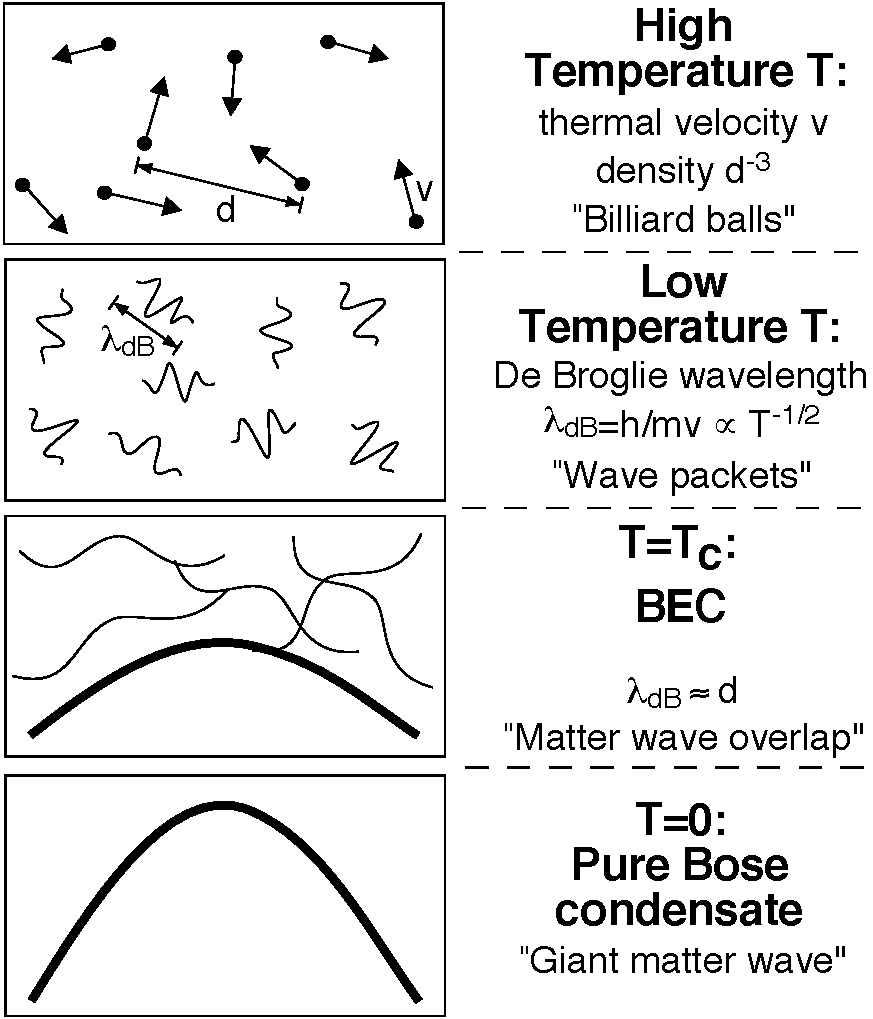
\includegraphics[width=8cm]{WhatIsBEC}
    \caption{
        \label{Introduction:WhatIsBEC}
        Comparison of the behaviour of a Bose gas at different temperatures.  See main text.  Reproduced from \citet{Ketterle:1999fk}.
    }
\end{figure}

The necessary property for the lasing mode of a laser --- be it optical or atomic --- is that it have an occupation much greater than one \citep{Wiseman:1997ba}.  For photons, such a highly-degenerate mode was first achieved with the development of the maser \citep{Gordon:1955}; a photon condensate cannot exist in equilibrium as total photon number is not conserved \citep{Muller:1986,Ketterle:1999fk}.  Total atom number is, however, conserved and Bose-Einstein condensation occurs below a critical temperature \citep{PethickSmith}.  Below this critical temperature, a significant fraction of the atoms in the system occupy a single spatial mode; exactly what is required of the lasing mode of an atom laser.

The process of Bose-Einstein condensation can be understood in a simplified picture in which the atoms are viewed as wave-packets with an extent of the order of the thermal de Broglie wavelength $\lambda_\text{dB} = (2 \pi \hbar^2 / M k_B T)^{1/2}$, where $M$ is the mass of the atom, $k_B$ is Boltzmann's constant, and $T$ is the temperature of the atoms.  At room temperature, the de Broglie wavelength is sufficiently small ($\sim 5\times\unit[10^{-11}]{m}$ for \nucl{4}{He} at $T=\unit[300]{K}$) that the atoms behave as point-like billiard balls (upper panel of \figureref{Introduction:WhatIsBEC}).  As the temperature decreases, the de Broglie wavelength increases (second panel of \figureref{Introduction:WhatIsBEC}).  As the temperature continues to decrease, the de Broglie wavelength approaches the mean interparticle separation $d$ and the atomic matter waves begin to overlap (third panel of \figureref{Introduction:WhatIsBEC}).  Below this temperature, a Bose-Einstein condensate begins to form, until at $T=\unit[0]{K}$, all atoms are in the condensate (lower panel of \figureref{Introduction:WhatIsBEC}).  Conservation of total number is necessary for BEC, as it is because of this that the interparticle separation $d$ remains constant as temperature is decreased (in a box of constant volume); for photons, as the temperature is decreased the total number of photons in the system decreases, increasing the mean interparticle separation $d$ faster than the photon wavelength increases.  Hence photon condensation cannot occur in equilibrium.

Bose-Einstein condensation is a macroscopic quantum phenomenon with a broad range of applications beyond the production of atom lasers.  Perhaps the most interesting of these are the development of \emph{quantum simulators} \citep{Lewenstein:2007,Buluta:2009}, experiments which directly realise theoretical condensed matter models, which were initially proposed as approximations to other systems.  For example, the Bose-Hubbard model \citep{Fisher:1989} of interacting bosons was realised by loading a BEC into an optical lattice.  By changing the depth of the optical lattice, the ratio of the tunnelling and interaction terms was changed, permitting direct observation of the superfluid to Mott-insulator transition \citep{Greiner:2002lr}.  Quantum simulators are possible for a variety of other systems, including Josephson junctions \citep{Levy:2007vn}, and reduced-dimension systems such as the Tonks-Girardeau model of 1D hard core bosons \citep{Girardeau:1960,Lieb:1963,Paredes:2004}.  Dilute gas BECs have also been used in the direct observation of persistent currents in the form of vortices and vortex lattices \citep{Abo-Shaeer:2001}, the coherent control of optical information \citep{Ginsberg:2007fk}, the observation of quantum optical effects in atoms such as the Hanbury-Brown-Twiss effect \citep{Jeltes:2007fk}, and four-wave mixing \citep{Deng:1999qy}.

% Theoretical things not included in the above list:
% realisation of an analogue to a magnetic monopole \citep{Pietila:2009}
% super-chemistry \citep{Heinzen:2000}: perform a chemical reaction in a controlled way, from a desired initial state to a desired final quantum state
% GR-analogues

% Other things not mentioned:
% Testing Bogoliubov's theory for excitations and the speed of sound (temperature dependence too)

One of the advantages of dilute gas BEC that gives these systems such a broad range of applications is the extraordinary degree to which these systems can be controlled and manipulated:  their effective dimensionality can be changed by changing shape of the confining potential \citep{Olshanii:1998,Paredes:2004,Kinoshita:2004}; the de Broglie wavelength is controllable over many orders of magnitude $\unit[1]{nm} \lesssim \lambda_\text{dB} \lesssim \unit[10]{\micro m}$; the sign and magnitude of interparticle interactions can be controlled \citep{Inouye:1998hy}, from attractive interactions through to almost infinitely repulsive interactions, including the non-interacting limit; essentially `pure' potentials (minimal absorption) may be constructed in a range of forms, including highly regular potentials such as harmonic or lattice potentials and random potentials with controllable statistical properties \citep{Damski:2003,Lye:2005,Clement:2005,Fort:2005,Schulte:2005}.  Dilute gas BEC also has a range of available observational tools for probing the system \citep{Ketterle:1999fk} including absorptive imaging, phase-contrast imaging, Bragg scattering \citep{Stenger:1999a}, and ion detection for metastable species \citep{Robert:2001}.

The goal of atom optics is to use the fundamental differences between atoms and photons in the application of the principles of laser optics to new fields of research.

\subsection{The outcoupling process}

The outcoupling of light from the lasing mode of a photon laser is achieved by making one of the cavity mirrors partially transparent.  The emitted light is the output mode of the photon laser.  For atom lasers, an analogous technique can be used in optical traps by lowering the depth of the trap until some atoms can tunnel out of the trap with the assistance of gravity.  In magnetic traps, electromagnetic radiation is applied to transfer the atoms (either directly with radio-frequency radiation \citep{Mewes:1997,Bloch:1999mi}, or indirectly via a multi-photon Raman transition \citep{Moy:1997,Hagley:1999dz,Robins:2006fk}) into a magnetically-insensitive state in which they fall freely under gravity.  These outcoupled atoms form the atom laser beam.

Contemporary atom optics experiments operate in pulsed mode.  Without a pumping mechanism, the atom laser beam is limited by the size of the condensate.  Once all of the atoms in the BEC have been outcoupled, the atom laser beam stops.  This places a fundamental limit on the linewidth (related to the longitudinal velocity-spread) of the atomic pulse produced: the Fourier limit, proportional to the inverse of the outcoupling time \citep{Johnsson:2007}.  This limit can be made arbitrarily small (until the energy uncertainty in the BEC due to interatomic scattering becomes significant \cite{Johnsson:2007a}) at the expense of an arbitrarily low atom flux.  Practically however, this trade-off cannot be made because the signal-to-noise ratio for atom laser experiments depends critically on the atomic flux \citep{Dowling:1998}.  The only way to achieve a high-flux atom laser with a narrow linewidth is with a continuous pumping process, which has yet to be achieved experimentally. 

The outcoupling process for atom lasers displays a range of behaviour.  While intuitively one might expect that increasing the outcoupling strength would continuously increase the atom laser flux, this is only true up to a point.  In the limit of large outcoupling rates, a bound state forms \citep{Jeffers:2000rr}, and the atom laser shuts down \citep{Robins:2004pz}.  

The outcoupling process also strongly affects the transverse profile of the atom laser.  Due to the mean-field repulsion the atoms experience as they leave the condensate, significant interference fringes are observed on the atom laser profile \citep{Busch:2002zr,Kohl:2005fk}.  These interference fringes complicate the spatial profile of the atom laser, making any atom interferometry experiment that relies upon separated beam paths more challenging.  The interference fringes on the transverse profile increase the sensitivity of the experiment to imperfections in the spatial overlap of the previously-separated beams when they are combined for detection.  These interference fringes may be reduced by outcoupling from the bottom of the condensate \citep{Riou:2006uq} or by giving the atoms a significant momentum kick as they leave the condensate \citep{Jeppesen:2008}.  The transverse profile of the atom laser is discussed in greater detail in \sectionref{BackgroundTheory:TransverseProfile}.

Even in the absence of a pumping process, atom lasers can be used for a variety of interesting experiments.  The correlation and counting statistics of an atom laser have been measured \citep{Ottl:2005}, an atom laser has been guided with optical waveguides \citep{Guerin:2006mz}, and a BEC has been probed using an atom laser outcoupled from a separate BEC \citep{Doring:2008}.  There have also been interesting theoretical proposals to produce non-classical atom laser states using the interatomic interaction of the atom laser \citep{Johnsson:2007b}, or by outcoupling with squeezed light \citep{Haine:2005}.  There is even a related proposal to generate controllable atom--light entanglement \citep{Haine:2006}.

% Comparison of multistate and two-state atom laser output couplers \citep{Dugue:2007fk}
% Quasi-monomode guided atom laser \citep{Couvert:2008}
% 
% Quantum-noise limits to the atom-laser gyroscope \citep{Dowling:1998} --- Perhaps this should go earlier?
% 
% First experimental studies of the divergence of the atom laser \citep{Le-Coq:2001vn}.
% Reducing the linewidth via feedback: \citep{Wiseman:2001zr}
% Bragg diffraction of an atom laser by an optical standing wave \citep{Wu:2006fj}
% It is claimed that gravitational wave detectors based on matter-wave interferometers are no better than laser interferometers \citep{Roura:2006}.
% Comparison of multistate and two-state atom laser output couplers \citep{Dugue:2007fk}
% Observation of transverse interference fringes: \citep{Dall:2007}
% Coherent splitting of an atom laser beam: \citep{Dugue:2008}
% Theoretical tools for atom laser beam propagation: \citep{Riou:2008}
% Quasi-monomode guided atom laser \citep{Couvert:2008}
% Two-state Raman outcoupler \citep{Debs:2009}

\subsection{The pumping mechanism}
\label{Introduction:ThePumpingMechanism}

\subsubsection{The photon laser}

The pumping mechanism of a laser acts as an amplifier for the lasing mode.  It is what replenishes the losses of the lasing mode due to outcoupling and any other loss processes.  Without a pumping mechanism, an optical laser is simply a leaky cavity emitting an exponentially-decreasing amount of light.  The linewidth of this emitted light is limited by the linewidth of the optical cavity.  The pumping mechanism for an optical laser not only permits continuous operation of the laser, it also narrows the linewidth of the laser in a process known as \emph{gain-narrowing}.  Gain-narrowing results from the saturation of the pumping process for large signals; no physical amplifier can amplify a signal indefinitely.  

\begin{figure}
    \centering
    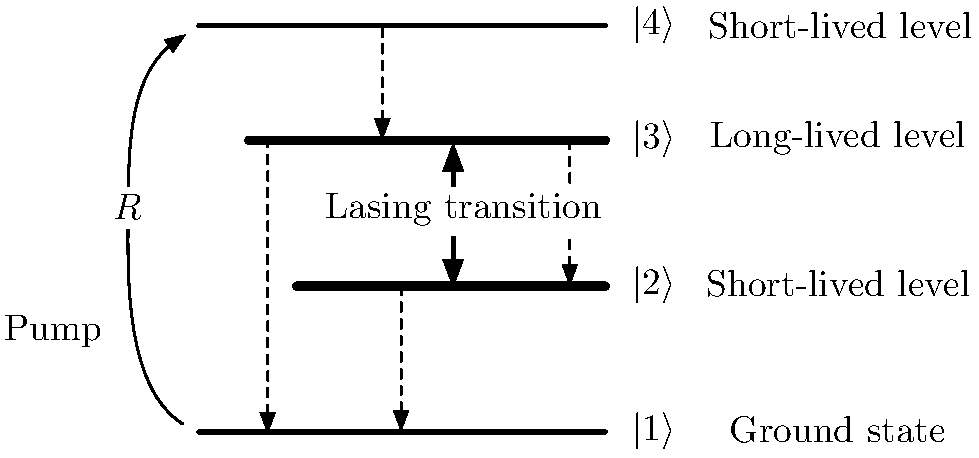
\includegraphics[width=8cm]{4LevelOpticalLaserModel}
    \caption{
        \label{Introduction:4LevelOpticalLaserModel}
        Schematic diagram of the atomic levels of a 4-level photon laser.  The dashed lines indicate decay processes, and the `slow' and `fast' labels indicate the relative speed of the decay processes.  Once atoms decay to the $\ket{1}$ ground state, they are pumped to the state $\ket{4}$ with a rate $R$.  This process drives the population inversion on the $\ket{2} \leftrightarrow\ket{3}$ transition.  Diagram derived from Figure~13.2-6 of \citet{SalehTeich}.
    }
\end{figure}

A pumping mechanism contains excitations that can each increase the occupation of the lasing mode by one.  These excitations are replenished at a finite rate, limiting the rate at which the lasing mode may be increased.  For example, in the 4-level photon laser model illustrated in \figureref{Introduction:4LevelOpticalLaserModel}, atoms are pumped from the ground state $\ket{1}$ to the short-lived state $\ket{4}$ at a rate $R$.  The atoms in state $\ket{4}$ may decay into the $\ket{3}$ state, the excited state of the lasing transition.  The occupation of the lasing mode cannot therefore be increased at a rate greater than $R$.  Any physical pumping mechanism will also exhibit saturation, and therefore the lasing mode will exhibit gain-narrowing.

Another necessary property of the pumping mechanism is that it be irreversible; once the occupation of the lasing mode has been increased, the probability that the process will reverse should be negligible.  This is achieved by coupling to a large number of essentially-empty modes known as a \emph{reservoir}.  In the case of the 4-level photon laser model depicted in \figureref{Introduction:4LevelOpticalLaserModel}, once an atom in the excited state $\ket{3}$ of the lasing transition has undergone stimulated emission into the $\ket{2}$ state by emitting a photon into the lasing mode, it rapidly decays into the ground state $\ket{1}$.  By ensuring that the ground state of the lasing transition $\ket{2}$ decays to the true ground state $\ket{1}$ faster than it can absorb a lasing photon, the pumping process is made irreversible.  The reservoir is comprised of the essentially-empty modes of the optical field coupled to the $\ket{1} \leftrightarrow \ket{2}$ transition, as once a photon on this transition is emitted spontaneously, it does not return.  This reservoir ensures that the modes of the $\ket{2}$ atomic level are also essentially empty.

Finally, in many circumstances it is desirable that the photon laser have only one lasing mode.  If the resonator supports many different modes, and if the gain bandwidth of the pumping mechanism encompasses more than one of these modes, multiple lasing modes may result.  As the photon--photon interaction is negligible, these lasing modes do not directly interact, and may operate independently.  Multiple-mode operation in a photon laser is naturally suppressed if the pumping process is \emph{homogeneously broadened}.  In homogeneously broadened gain media, every excitation of the pumping mechanism contributes to the gain of the lasing modes in the same way, i.e.\ every excitation is resonant with the same lasing modes.  If the gain medium is \emph{inhomogeneously broadened}, some classes of pumping excitations will contribute differently to the total gain profile than others.  A classic example of this is Doppler-broadening.  Atoms in a gain medium have a finite temperature, and their motion affects what frequencies they are resonant with (in the laboratory frame) due to the Doppler effect.  If the size of this frequency broadening is greater than the natural linewidth of the lasing transition, not all of the pumping excitations will be resonant with a given lasing mode.  It will therefore only be those pumping excitations resonant with a given lasing mode that are saturated by it; lasing modes resonant with the remaining unsaturated pumping excitations will continue to experience gain and may lase independently.  In this case, thse lasing modes will experience gain independently, each without saturating the other.  If the pumping process is inhomogeneously broadened, undesirable modes can be removed by increasing their loss in the optical resonator.  This is naturally achieved by the addition of a second, smaller cavity inside the resonator that is only resonant with the desired mode.  If the pumping process is homogeneously broadened however, while multiple modes may initially experience gain, only the mode with the largest net gain will survive as the gain saturates, resulting in single-mode operation.


\subsubsection{The atom laser}

\begin{figure}
    \centering
    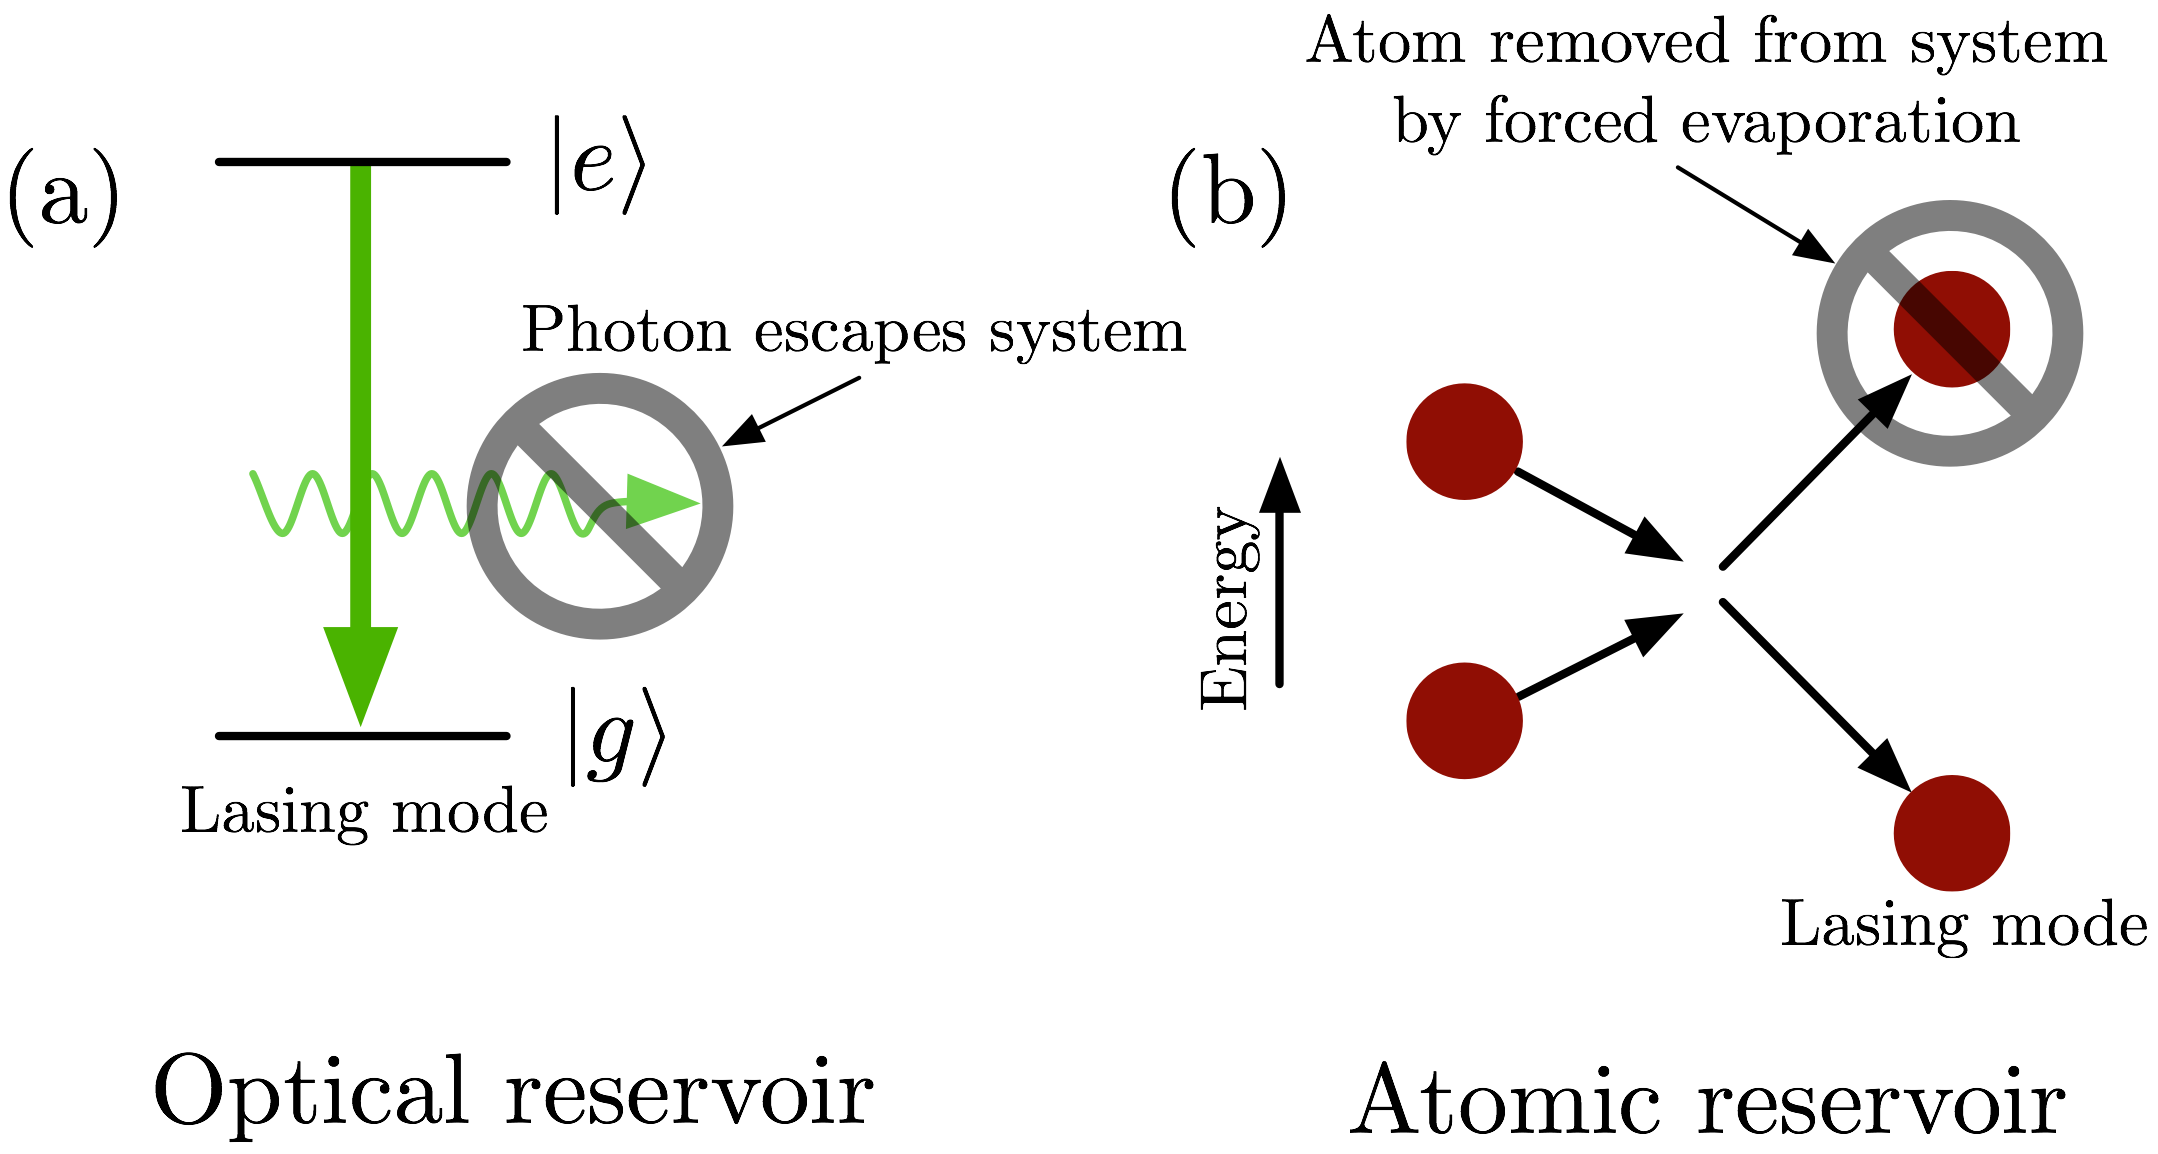
\includegraphics[width=10cm]{ReservoirChoices}
    \caption{
        \label{Introduction:ReservoirChoices}
        Classes of pumping mechanism for an atom laser as defined by the reservoir.  The crossed circle indicates which excitation in the process irreversibly leaves the system.
    }
\end{figure}

There are two choices of reservoir for the pumping mechanism of an atom laser: the empty modes of the optical field, or the empty modes of the atomic field.  Each choice corresponds to a different class of pumping mechanism.  These two classes are illustrated in \figureref{Introduction:ReservoirChoices}.  In the first, an atom in an excited internal state is brought into resonance with the lasing mode such that it can decay into the lasing mode.  It is Bose-stimulated to do so by the occupation of the atomic lasing mode.  Once the emitted photon leaves the system, this decay is irreversible.  In the second, two atoms scatter into different energy states, one going into the lasing mode, while the other gains sufficient energy to be removed from the system (for example, due to forced evaporation, the same process used in the formation of BEC).

Single-mode operation is not simply desirable for an atom laser, it is necessary.  Due to the large interatomic interactions, multiple lasing modes in an atom laser could not operate independently.  Significant scattering would occur between the lasing modes, increasing the linewidth of both, possibly destroying any laser-like qualities in the process.  While the interatomic interactions can be `switched off' with the use of a Feschbach resonance \citep{Inouye:1998hy}, the loss processes are such that higher energy modes experience \emph{less} loss than the lower modes in this case, making the atom laser unstable \citep{Haine:2002kp}.  This instability can be resolved by increasing the interatomic interactions \citep{Haine:2002kp}, adding a position-dependent loss near the edge of the lasing mode \citep{Kneer:1998fk}, and in the case of non-zero interatomic interactions, by increasing the pumping rate \citep{Robins:2001pd}.

In all of the phenomenological atom laser pumping models discussed in the previous paragraph, the gain mechanism was effectively `homogeneously broadened' in the sense that all pumping excitations contributed equally to the gain of all modes.  This is more difficult to achieve for atom lasers than for photon lasers.  In the case of photon lasers, the dispersion relation for the by-product of the gain process (the de-excited atom) is relatively flat by comparison to that of the lasing mode.  This is a useful property, as it means that pumping excitations with a wider range of momenta are resonant with the lasing mode, as variations in the momentum difference between the pumping excitation and the lasing mode can be compensated for by the by-product with minimal energy cost.  In the limit of a perfectly flat dispersion relation for the by-product, pumping excitations of any momentum can result in gain if the decay process conserves energy, and due to the finite linewidth of the transition, energy need only be conserved to within this energy uncertainty.  As a concrete example, consider the photon laser pumping mechanism illustrated in \figureref{Introduction:4LevelOpticalLaserModel} and the atom laser pumping mechanism illustrated in \figureref{Introduction:ReservoirChoices}(a).  The fundamental difference between these two pumping mechanisms is that for the photon laser, the emitted photon goes into the lasing mode with the atom as the by-product, while for the atom laser, it is the decayed atom that enters the lasing mode with the emitted photon as the by-product.  The decay process of these pumping mechanisms is illustrated in \figureref{Introduction:AtomDecay}.  If a violation of energy conservation is permitted in this process of up to $\pm \hbar\Delta\omega$ where $\Delta\omega$ is the linewidth of the $\ket{g} \leftrightarrow \ket{e}$ transition, excited atoms with a wider range of momenta can contribute gain to the lasing mode in the case of the photon laser than in the case of the atom laser.  Specifically, for the photon laser, the wavenumber of the excited atom in the direction parallel to the lasing mode may vary by
\begin{align*}
    \left(\Delta k_{i,\parallel}\right)_\text{ph} \approx \frac{2 M \Delta\omega}{\hbar \abs{\vect{k}_\gamma}},
\end{align*}
where $M$ is the mass of the atom.  The wavenumber of the atom in perpendicular directions is unconstrained.  However, for the atom laser, the magnitude of the wavenumber of the excited atom may only vary by (assuming a stationary lasing mode of size $d$)
\begin{align*}
    \left(\Delta \abs{\vect{k}_{i}}\right)_\text{at} \approx \frac{2 \Delta\omega}{c} + \frac{\pi}{d},
\end{align*}
where the second term is due to the momentum-width of the lasing mode.  For the $\lambda = \unit[633]{nm}$ lasing transition of the Helium-Neon gas laser, $\Delta\omega \approx \unit[100]{MHz}$ \citep{SiegmanLasers}, $M_\text{Ne} = 3.3 \times \unit[10^{-26}]{kg}$, giving $\left(\Delta k_{i,\parallel}\right)_\text{ph} \sim \unit[10^{10}]{m\textsuperscript{-1}}$ for the photon laser and $\left(\Delta \abs{\vect{k}_{i}}\right)_\text{at} \sim \unit[10^{6}]{m\textsuperscript{-1}}$ for an atom laser with a lasing mode of size $d \sim \unit[10]{\micro m}$.  This difference significantly constrains the possible momentum width of the pumping excitations for the pumping mechanism to operate in the `homogeneously broadened' limit.  If the momentum width of the pumping excitations is greater than this, gain for modes other than the main lasing mode will not be saturated by the main lasing mode.  The remaining modes experiencing gain will increase the linewidth of the atom laser.

\begin{figure}
    \centering
    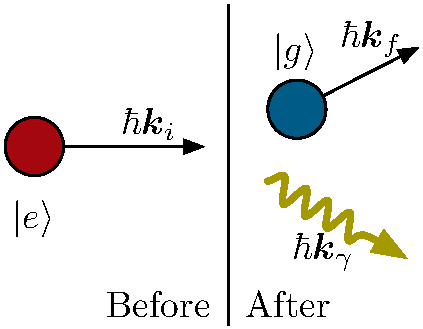
\includegraphics[width=6cm]{AtomDecay}
    \caption{
        \label{Introduction:AtomDecay}
        Excited state atom in the $\ket{e}$ state with momentum $\hbar \vect{k}_i$ decays into an atom in the ground state $\ket{g}$ with momentum $\hbar \vect{k}_f$, and a photon with momentum $\hbar \vect{k}_\gamma$.  In the photon laser pumping mechanism, the photon is in the lasing mode and the atom decays into a mode that is essentially unoccupied (the atom is the by-product of the gain process), while in an atom laser pumping mechanism, the decayed atom is in the lasing mode and the emitted photon is part of the reservoir which is essentially unoccupied (the photon is the by-product of the gain process).
    }
\end{figure}

In \chapterref{OpticalPumping}, a pumping mechanism for an atom laser using an optical reservoir is considered.  We attempt to solve the problem of the narrow permissible momentum width of the pumping excitations by making their momentum distribution sufficiently narrow that it can be guaranteed that every atom will be momentum-resonant with the pumping process at some point.  

In \chapterref{KineticTheory}, a pumping mechanism using atomic modes as the reservoir is considered.  Although their dispersion relation cannot be considered flat with respect to that of the lasing mode atoms, it is far more so than that of the photons.  The difficulty with this pumping mechanism is that it is inescapable that thermal atoms will be in the vicinity of the lasing mode.  Scattering between the lasing and thermal atoms will contribute to the collisional broadening of the lasing mode.  Using a Feschbach resonance to cancel these interactions is not an option as the pumping mechanism itself relies upon interatomic collisions.

\section{Matter wave amplification\dots}

A number of matter-wave amplification processes using the two possible reservoirs have been proposed and demonstrated.  These are discussed in this section.  While none of these matter-wave amplification processes constitute an atom laser pumping mechanism, it is envisaged that an atom laser pumping mechanism would be based on a similar process.

\subsection{\dots\ using an optical reservoir}

A number of previous experiments observing the process of super-radiant Rayleigh scattering seem to offer a physical mechanism for providing pumping through matter-wave amplification \citep{Inouye:1999ph,Kozuma:1999pi}.  Super-radiant Rayleigh scattering occurs when a far off-resonant laser illuminates an elongated BEC.  A matter-wave grating forms along the long axis of the BEC and atoms are preferentially scattered into non-stationary momentum states.  By providing a moving `seed', researchers were able to demonstrate pulsed coherent amplification via the Rayleigh super-radiance mechanism.  However, this type of matter-wave amplification is a transient phenomena, observed over timescales ranging from tens \citep{Inouye:1999ph} to hundreds of microseconds \citep{Kozuma:1999pi}.  On longer timescales, scattering into successively higher momentum modes seems unavoidable \citep{Zobay:2006}, resulting in a `fan'-shaped scattering pattern \citep{Inouye:1999yq}.

Two promising mechanisms for providing a pumping mechanism consistent with a continuous atom laser have recently been demonstrated.  The first is far-detuned stimulated Raman scattering \citep{Schneble:2004,Yoshikawa:2004}, in which atoms in one internal atomic state are Bose-stimulated to make transitions into an alternative atomic state.  The second, reported by \citet{Ginsberg:2007fk}, is a resonant coupling driven by electromagnetically-induced transparency (EIT), demonstrated as stimulated decay of atom pulses into a condensate in a freely falling frame.  In both cases, the coupling from the source mode is irreversible and the laser mode is dark to the photons produced by the stimulated transitions.

In \chapterref{OpticalPumping}, we consider a pumping mechanism for an atom laser derived from the Raman superradiance and EIT matter-wave amplification processes.  A discussion of related theoretical proposals is given in that chapter.

% \subsubsection{Theoretical proposals}
% 
% There have been several theoretical proposals for atom laser pumping mechanisms that use optical reservoirs.  Several of these\footnote{FIXME: Missing citations.} operate in the Lamb-Dicke limit in which the lasing mode is significantly smaller than the wavelength of the photons they emit.  This is a difficult regime to reach, and it requires the use of a Feschbach resonance to make interatomic interactions negligible if the lasing mode is to be operated with even relatively modest lasing mode occupations $N_0 \gtrsim 10^2$ \citep{Cirac:1994}.  This is an experimental difficulty, but not an insurmountable one.  There are other difficulties with these proposals that are more fatal.
% 
% \citet{Spreeuw:1995} propose trapping atoms in a repulsive optical lattice.  Loss due to off-resonant scattering from the optical trapping beams is greater for the higher-energy states of each lattice site as these states penetrate the repulsive trapping potential more than the lower-energy states.  This gives this proposal the favourable property that loss from higher-energy states is greater than that for lower-energy states, a property difficult to achieve in some circumstances (see \sectionref{Introduction:ThePumpingMechanism}).  However, this proposed pumping mechanism requires that the characteristic energy of the thermal source atoms $k_B T \lesssim \hbar \omega$, where $\omega$ is the trapping frequency of the lattice sites.  As this is also the energy separation between the trapped levels, this must be significantly less than the trap depth, thus requiring that the thermal clouds be isolated to each lattice site.  Each lattice site would therefore operate as independent atom lasers with random relative phases.  The outcoupled mode from this system would therefore not have the coherence properties desired of an atom laser.
% 
% \citep{Cirac:1994} consider a closed system, and optical cooling of a thermal cloud in a system in the LDL.  
% 
% 
% The desire in the LDL is to optically cool to form an atom laser
% 
% \citep{Cirac:1994} is another model in the LDL, which is based upon coherent pumping, and spontaneous decay.  It is also necessary that the degeneracy of the levels is lifted such that reabsorption is not a problem.  This requires that $\Gamma \ll \omega_\text{trap}$, which is a significant requirement.
% 
% A model for an atom laser \citep{Olshanii:1996} --- Single mode, effective Homogeneous broadening, optical pumping.  Sort of phenomenological model that neglects reabsorption.  Considering the opposite limit to the LDL, but quite phenomenologically.
% 
% Cirac and Lewenstein BAR model \citep{Cirac:1996rr}.  Incoherent pumping, then decay driven.
% 
% Continuous optical loading of a Bose-Einstein condensate \citep{Santos:2001ve} --- Few mode model, Homogeneous broadening.  Optical pumping.


\subsection{\dots\ using an atomic reservoir}

The production of BEC using the standard technique of evaporation \citep{Hess:1986,Ketterle:1996} is a matter-wave amplification process \citep{Luiten:1996,Gardiner:1997uq,Miesner:1998}.  In this process, atoms with energy greater than a threshold are removed from the system, thus reducing the mean energy of the system.  Elastic collisions between the remaining atoms lead to rethermalisation at a lower temperature.  This process has been experimentally demonstrated to give exponential gain of the condensate mode until the thermal cloud becomes significantly depleted \citep{Miesner:1998}.

Four-wave mixing of matter-waves \citep{Deng:1999qy} is a fundamentally similar process in which two atoms undergo a collision and scatter into different momentum modes.  When one of the final momentum modes is already occupied, this process is Bose-enhanced, and is a matter-wave amplification process \citep{Vogels:2002}.  If neither of the final momentum modes are occupied, the scattering process gives rise to entanglement between the atoms in the final momentum modes, although only classical correlations have been observed to date \citep{Perrin:2007}.

In \chapterref{KineticTheory}, we consider a pumping mechanism for an atom laser driven by evaporation.  In particular, we consider the temperature and flux requirements of the atomic source that must be used to replenish the thermal cloud.


% Theory of an atom laser \citep{Holland:1996mz} --- Single mode, effective Homogeneous broadening, it works, evaporative pumping
% An atom laser based on evaporative cooling \citep{Wiseman:1996} --- Single mode, effective Homogeneous broadening, it work, evaporative pumping
% Theory of a coherent atomic-beam generator \citep{Guzman:1996} ---  Atoms trapped in an optical lattice, interacting via the dipole-dipole interaction.  This dipole-dipole interaction is mediated by the optical lattice.  The dipoles are in fact formed by the optical lattice.  Absent the ac Stark shift, the dipole-dipole interaction would be negligible.  The dipole-dipole interaction therefore occurs whenever \emph{detuned} radiation is present.  In the presence of resonant light, it may be that other effects dominate.  Their simulations are effectively single mode, effective Homogeneous broadening, dipole--dipole interaction with evaporative pumping
% Reducing the Linewidth of an Atom Laser by Feedback \citep{Wiseman:2001zr} --- Single mode model, but demonstrates that some of the linewidth issues can be resolved by feedback
% More feedback reducing the linewidth \citep{Thomsen:2002xc}.

\section{Thesis overview}

In this thesis, we focus on an investigation of atom laser pumping mechanisms, both using an optical reservoir, which is discussed in \chapterref{OpticalPumping}, and with an atomic reservoir, which is discussed in \chapterref{KineticTheory}.  In \chapterref{Peaks}, we discuss an unusual process in which atomic interaction energy is directly converted into kinetic energy, potentially leading to the formation of entangled atomic beams.  An overview of the common theoretical tools and techniques is given in \chapterref{BackgroundTheory}, and concluding remarks to the thesis are given in \chapterref{Conclusion}.

\parasep

The following is a list of publications written as part of the author's PhD.
\begin{enumerate}
    \item `\emph{Observation of transverse interference fringes on an atom laser beam}'; R.~G.~Dall, L.~J.~Byron, A.~G.~Truscott, G.~R.~Dennis, M.~T.~Johnsson, M.~Jeppesen, and J.~J.~Hope, Opt.~Express \textbf{15}, 17673 (2007).
    \item `\emph{Multibeam atom laser: Coherent atom beam splitting from a single far-detuned laser}'; J.~Dugué, G.~Dennis, M.~Jeppesen, M.~T.~Johnsson, C.~Figl, N.~P.~Robins, and J.~D.~Close, Phys.~Rev.~A \textbf{77}, 031603 (2008).
    \item `\emph{A pumped atom laser}'; N.~P.~Robins, C.~Figl, M.~Jeppesen, G.~R.~Dennis, and J.~D.~Close, Nat.~Phys. \textbf{4}, 731 (2008).
    \item `\emph{Approaching the Heisenberg limit in an atom laser}'; M.~Jeppesen, J.~Dugué, G.~R.~Dennis, M.~T.~Johnsson, C.~Figl, N.~P.~Robins, and J.~D.~Close, Phys.~Rev.~A \textbf{77}, 063618 (2008).
    \item `\emph{Paired-atom laser beams created via four-wave mixing}'; R.~G.~Dall, L.~J.~Byron, A.~G.~Truscott, G.~R.~Dennis, M.~T.~Johnsson, and J.~J.~Hope, Phys.~Rev.~A \textbf{79}, 011601 (2009).
    \item `\emph{Pulsed pumping of a Bose-Einstein condensate}'; D.~Döring, G.~R.~Dennis, N.~P.~Robins, M.~Jeppesen, C.~Figl, J.~J.~Hope, and J.~D.~Close, Phys.~Rev.~A \textbf{79}, 063630 (2009).
    \item `\emph{Creating EPR entangled matter beams via instabilities in Bose-Einstein condensates}'; G.~R.~Dennis and M.~T.~Johnsson, in preparation (2010).
    \item `\emph{Quantum kinetic theory model of a continuous atom laser}'; G.~R.~Dennis, M.~Davis, and J.~J.~Hope, in preparation (2010).
\end{enumerate}
In this thesis, the work of papers 1, 3, and 5--8 are presented.  Specifically, the work of paper 1 is presented in \sectionref{BackgroundTheory:TransverseProfile}, that of papers 5 and 7 are presented in \chapterref{Peaks}, that of papers 3 and 6 is presented in \chapterref{OpticalPumping}, and that of paper 8 is presented in \chapterref{KineticTheory}.
